\scanpage{18}
\handwritten{\mspage{9}}
\margin{\handwritten{\unsure{non}, pas tout à fait !}}
7. Je \rlap{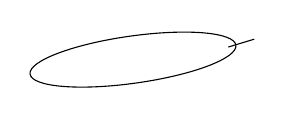
\begin{tikzpicture}[x=1cm,y=1cm,baseline=-0.45ex]\draw[rotate=8] (1.23,0.06) ellipse (1.32cm and 0.30cm);\draw (2.42,0.39)--(2.75,0.49);\end{tikzpicture}}vais prouver la conjecture du n°6 pour des pinceaux de Lefschetz \deleted{\uline{Théorème}} assez généraux d'hypersurfaces de grand degré, en adaptant la méthode utilisée par Katz pour les intersections complètes. Nous allons prouver:

\margin{\handwritten{\unsure{pas prouvé} \unsure{sous cette} forme forte}\figure{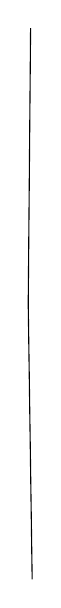
\begin{tikzpicture}[x=1cm,y=1cm]\draw (0.05,0)--(0,3.5)--(0.03,7);\end{tikzpicture}}}
\uline{Théorème} 7.1. Soit $X\handwritten{\subset}P^r_k$ un schéma projectif équidimensionnel de Cohen-Macaulay, de dimension $n\handwritten{>}0$, sur un corps $k$ de car. $p\handwritten{>}0$. Il existe alors un entier $d_o\handwritten{>}0$ tel que, pour tout $d\handwritten{\geq}d_o$, si $Y$ est la section de $X$ par l\deleted{'}a\deleted{section} hypersurface générique de degré $d$, définie sur l'extension $k'=k(t_o,..,t_r)$ de $k$, on ait la propriété qui suit\deleted{e}. On désigne par $E_o(Y)$ le conoyau de $H^{n-1}(X_{k'},\underline{O}_{X_{k'}})\handwritten{\longrightarrow}H^{n-1}(Y,\underline{O}_Y)$, qui est \deleted{muni d'un} un vectoriel de dimension finie sur $k'$, muni\deleted{e} de l'homomorphisme $p$-linéaire de frobenius $E_o(Y)^{(p)}\handwritten{\longrightarrow}E_o(Y)$ (prov\deleted{\unsure{t|i}}enant de la puissance p.ème sur les faisceaux de coéfficients $\underline{O}_{X_{k'}}$, $\underline{O}_Y$). Soit \inserted{$V=$}$E_o(Y)_{ss}$ la partie semi-simple de $E_o(Y)$, i.e. le plus grand sous-espace \inserted{$V$} stable par frobenius et sur lequel frobenius induise un morphisme surjectif $V^{(p)}\handwritten{\longrightarrow}V$.

Considérons la représentation correspondante de $\unsure{G'|G}=\mathrm{Gal}(\bar k'/k')$ dans le vectoriel \inserted{$V_o$} de di\deleted{\unsure{e}}m\deleted{\unsure{m}}ension $s=\dim_{k'}V$ sur $\underline{F}_p$ formé\deleted{\unsure{s|e}} des $x\handwritten{\in}V_{\bar k'}$ tels que $Fx=x$. Alors \deleted{cette représentation est non triviale, et de façon plus précise,} pour tout élément $a\handwritten{\in}\underline{F}^{\deleted{\handwritten{\unsure{*|\times}}}}_p$, il existe un $u\handwritten{\in}\mathrm{Aut}(V_o)$; dans l'image \inserted{$G_o$} de $G$\inserted{\handwritten{, et un sous-espace $V'_o\subset V_o$ stable par $\unsure{u|G_o|G}$,}} tel que $\mathrm{Tr}\ u\handwritten{|V'_o}=a$. \deleted{\handwritten{[}(Cela implique en particulier que $G_o$ n'est pas un $p$-groupe, et plus précisément qu'il a au moins $p\deleted{\unsure{-1|+1}}$ éléments distincts (\deleted{car}\inserted{et même} à traces distinctes) qui \deleted{\unsure{ne|xx}} sont semi-simples.\deleted{\unsure{)}}\inserted{\handwritten{Cela implique également que $s=\dim V\geq2$}}\handwritten{).]}}

Signalons tout de suite les corollaires qui nous intéresseront surtout:

\margin{\handwritten{\unsure{pas prouvé}; \unsure{est} équivalent \unsure{à} 7.1 sous sa forme forte}\figure{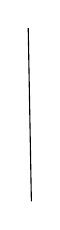
\begin{tikzpicture}[x=1cm,y=1cm]\draw (0.04,0)--(0,2.2);\end{tikzpicture}}}
\uline{Corollaire} 7.2. Supposons que $k$ soit fini. Soit $S_d$ le schéma projectif défini par le vectoriel des formes de degré $d$ sur $P^r_k$, Alors pour tout ouvert non vide $U$ de $S_d$, et tout entier $a$, il existe un \inserted{\handwritten{point \deleted{\unsure{fermé}}}} $t\handwritten{\in}U\handwritten{(k')}$ \deleted{tel que}\inserted{\handwritten{(\unsure{avec|où} $k'$ \inserted{une} extension finie de $k$) tel que}}
% archive sheet number: 17
